\documentclass[11pt]{article}
\usepackage{estilo}


\author{
    \begin{tabular}{c}
        Artur Gemaque Rezende da Silva, \\
        Engenharia Aeroespacial, UFSC, \\
        Campus Joinville, Santa Catarina, Brasil \\
        e-mail: eng.arturgemaque@gmail.com \\
    \end{tabular}
}
\date{}

\begin{document}

%-------------------- Cabeçalho Inicial --------------------%
\begin{center}\Huge\textbf{Trabalho de Física III}\end{center}
\smallskip

\begin{abstract}
    \noindent Neste trabalho, abordarei os princípios fundamentais do funcionamento do motor BLDC (Motor de Corrente Contínua sem Escova). 
    Diferentemente dos motores DC tradicionais, o BLDC utiliza um sistema eletrônico para a comutação da corrente, em vez de comutadores mecânicos, 
    resultando em maior eficiência e promovendo o aumento da vida útil do equipamento.

\end{abstract}

%-------------------- Texto --------------------%

\section{Introdução}
    \noindent Os motores BLDC (Brushless DC) são amplamente utilizados em sistemas que exigem alta rotação e baixo desgaste mecânico, 
    como na fabricação de drones e furadeiras, atuando na conversão de energia elétrica em energia mecânica. Para compreender os conceitos físicos que regem 
    seu funcionamento, é importante, inicialmente, analisar sua versão mais simples: o motor DC (motor de corrente contínua). A principal 
    diferença entre eles está no método de comutação da corrente, tema que será detalhado ao longo deste trabalho.

\begin{multicols}{2}
    
    \begin{figure}[H]
        \centering
        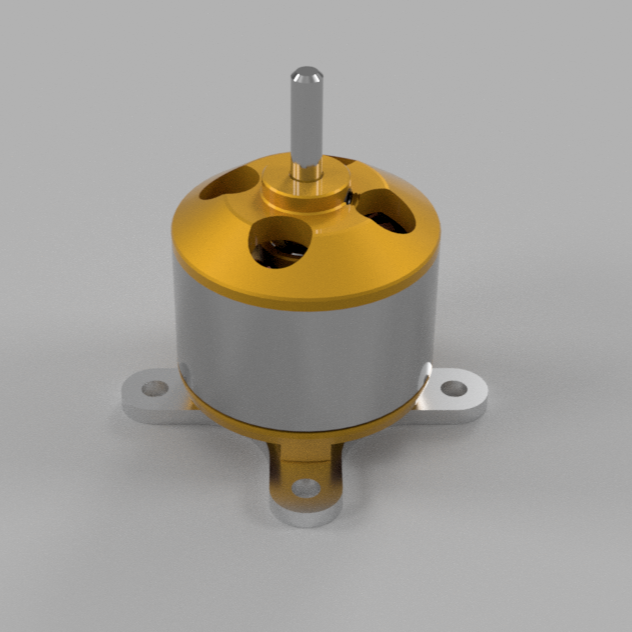
\includegraphics[width=5cm]{Renderizações/1 - BLDC.png}
        \caption{Exemplo Motor BLDC}
        \footnotesize \textit{Fonte: Renderização própria no Fusion 360.}
        \label{1-BLDC}
    \end{figure}

    \begin{figure}[H]
        \centering
        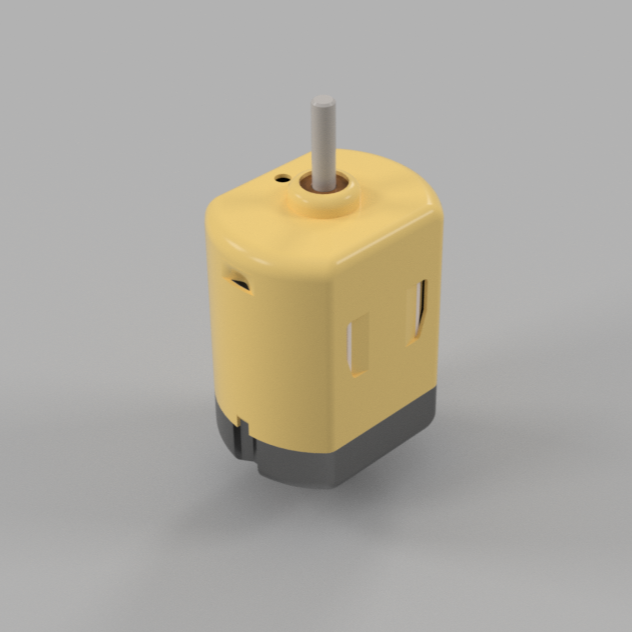
\includegraphics[width=5cm]{Renderizações/1 - DC.png}
        \caption{Exemplo Motor DC}
        \footnotesize \textit{Fonte: Renderização própria no Fusion 360.}
        \label{1-DC}
    \end{figure}

\end{multicols}

\section{Componentes Motor CC}

    \noindent Ao observar um motor DC, a primeira parte visível é a sua \textbf{carcaça}, responsável por fornecer suporte estrutural ao conjunto. 
    No centro, encontra-se o \textbf{eixo}, uma barra concêntrica ao motor que se estende de um dos lados e realiza transferência da energia mecânica. Já na 
    outra extremidade localizam-se os dois \textbf{terminais} destinados à alimentação elétrica.

    Removendo a carcaça, é possível identificar dois ímãs que compõem o \textbf{estator}, a parte que fica parada, estes são imãs permanentes que definem os polos norte e sul 
    magnéticos. Centralizado ao conjunto podemos ver novamente o eixo que está acoplado ao \textbf{rotor}, a parte do motor que efetivamente gira, formado por vários discos eletricamente 
    isolados entre si, geralmente em formato de "T". Nos braços do rotor, estão enroladas as \textbf{bobinas}, responsáveis por conduzir a corrente elétrica 
    proveniente da bateria. À medida que a corrente percorre as bobinas é possível controlar a velocidade e rotação do motor.

    \begin{multicols}{2}
    
    \begin{figure}[H]
        \centering
        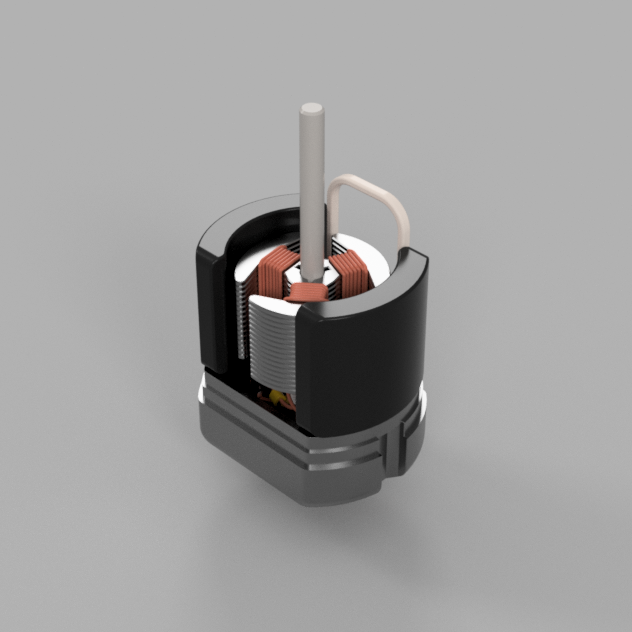
\includegraphics[width=5cm]{Renderizações/2 - DC.png}
        \caption{Motor DC interno}
        \footnotesize \textit{Fonte: Renderização própria no Fusion 360.}
        \label{2-DC}
    \end{figure}

    \begin{figure}[H]
        \centering
        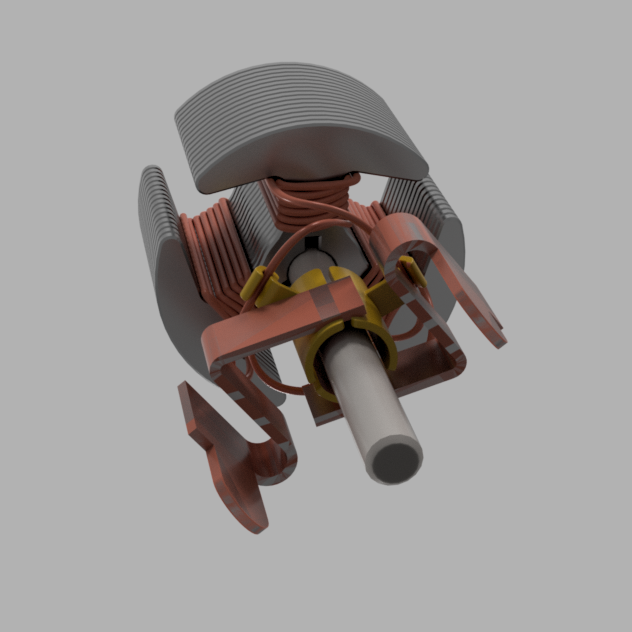
\includegraphics[width=5cm]{Renderizações/3.1 - DC.png}
        \caption{Motor DC Comutador}
        \footnotesize \textit{Fonte: Renderização própria no Fusion 360.}
        \label{3-DC}
    \end{figure}

    \end{multicols}

    As extremidades das bobinas são conectadas ao \textbf{comutador}, um anel segmentado composto por placas dispostas concentricamente ao redor do eixo, essas 
    placas são eletricamente isoladas entre si e do próprio eixo. Ao observar o lado interno da tampa que sustenta os terminais, encontram-se as \textbf{escovas} 
    e seus respectivos \textbf{braços}. O comutador é posicionado entre as duas escovas, que fazem contato com seus segmentos para completar o circuito elétrico. 
    O fluxo do circuito ocorre determina o sentido de rotação.

    \begin{center}
        Terminal (Positivo ou Negativo) \( \rightarrow \) Braço da Escova \( \rightarrow \) Escova \( \rightarrow \) Comutador \( \rightarrow \) Bobina \\
        Bobina \( \rightarrow \) Comutador \( \rightarrow \) Outra Escova \( \rightarrow \) Braço da Outra Escova \( \rightarrow \) Terminal Oposto
    \end{center}

\section{Princípios físicos por trás do motor CC}
    \noindent Ao analisarmos um circuito simples e conectarmos os terminais em uma bateria, os elétrons fluirão do terminal negativo para o positivo, 
    mesmo se criarmos um caminho temporário, eles o seguirão enquanto estiver disponível. Em uma situação qualquer os elétrons passaram pelo fio gerando 
    um campo eletromagnético ao redor do fio.

    Contudo este campo ainda é muito fraco para nossa aplicação nos motores DC e BLDC, por isso os fios são enrolados através do rotor. Cada fio cria um campo eletromagnético
    e juntos combinam suas linhas de campo paralelas em um campo magnético muito maior gerando assim uma bobina com campo magnético em seu 
    interior tendendo à uniformidade. Então podemos criar um campo magnético que age como um ímã permanente, exceto que com esse tipo conseguimos desligar e ligar o 
    campo.
    
    Para melhor compreensão do fenômeno da rotação vamos considerar um motor simplificado em que há dois ímãs fixos, um com polo norte e outro com polo sul, posicionados 
    em lados opostos. Entre eles, há uma bobina conectada a um circuito elétrico. Quando a corrente elétrica passa pela bobina, ela interage com o campo magnético dos ímãs, 
    gerando forças opostas em cada lado da bobina: de um lado, a força aponta para baixo; do outro, para cima. Esse par de forças cria um torque que faz a bobina girar, 
    ilustrando o princípio básico de funcionamento dos motores de corrente contínua. Quantificado pela equação:

    \begin{equation}
        \nonumber
        \label{eqlorentz}
        \vec{F} = q \,.\, ( \vec{v} \times \vec{B}) \;\;\; \rightarrow \;\;\; \vec{F} = I \,.\, (\vec{l} \times \vec{B})
    \end{equation}

    Entretanto, existe um desafio: à medida que a bobina gira, ela pode se alinhar com o campo magnético dos ímãs do estator, o que faz com que as forças se cancelem e a 
    rotação pare. Para evitar esse travamento, o motor utiliza o comutador, cuja principal função é inverter automaticamente o sentido da corrente elétrica 
    nas bobinas sempre que a bobina passar pela posição de alinhamento com o campo magnético. Essa inversão garante que a força resultante continue favorecendo a rotação, 
    impedindo o travamento do motor. 
    
    Assim, o comutador assegura que o fluxo de corrente seja alterado no momento exato para manter a geração de torque na direção desejada, além de que quanto mais conjuntos 
    de bobinas tivermos, mais suave será a rotação. Portanto, normalmente encontramos pelo menos 3 conjuntos de bobinas em um motor para garantir a rotação suave. Cada 
    bobina está conectada a duas placas comutadoras, placas eletricamente isoladas entre si, exceto pelo fato de serem conectadas através das bobinas. Assim, as escovas se 
    esfregam contra as placas do comutador podendo ligar as bobinas duas a duas nos terminais. Dessa forma criamos um motor simples.

    Vale a pena observar que as correntes de Foucault são reduzidas nos motores através do uso de laminações (chapas finas isoladas) no estator e rotor.
    Também conhecidas como correntes parasitas, são as correntes elétricas induzidas dentro de um material condutor, quando sujeito a um campo magnético variável. 
    Conforme a Lei de Lenz, a magnitude e sentido dessa corrente se opõe à variação do campo que a provoca, formando polos magnéticos que geram forças 
    que efetivamente se opõem ao movimento do material condutor dentro do campo magnético, realizando a frenagem do motor.
    
    \bigskip
    \bigskip

    \begin{figure}[H]
        \centering
        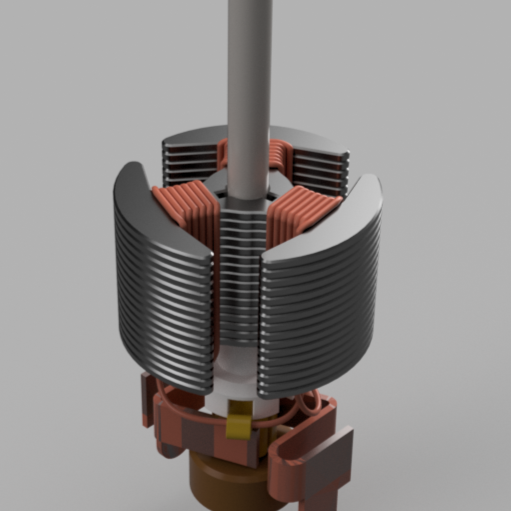
\includegraphics[width=7cm]{Renderizações/4 - DC.png}
        \caption{Motor DC Rotor}
        \footnotesize \textit{Fonte: Renderização própria no Fusion 360.}
        \label{4-DC}
    \end{figure}

\section{Componentes e Funcionamento do Motor BLDC}
    \noindent Quando comparamos Motor BLDC com o Motor DC podemos notar que ambos têm ímãs na parte interna da carcaça e bobinas de cobre no centro. Contudo, enquanto 
    os motores DC têm as escovas que se esfregam ao comutador utilizando blocos de carbono, os motores BLDC não as possuem, isso se deve ao design que permite as bobinas ficam no estator (parte estacionária) 
    e os ímãs permanentes no rotor (parte móvel), como não há escovas, quase não há atrito. Este motor utiliza três fios, cada fio representa uma fase e as fases duas a duas 
    ligam os 3 conjuntos de bobinas no interior do motor, por sua vez as bobinas são ligadas ao controlador eletrônico de velocidade, que tem como função 
    gerênciar a sequência de energização das bobinas, controla velocidade, sentido e garantir o funcionamento do circuito proteções.
    
    Assim como era no motor DC, quando um conjunto de bobina é energizado, cria os campos eletromagnéticos que interagem com os ímãs permanentes no rotor que causa a rotação. O controlador 
    irá receber um sinal eletrônico indicando a ordem em que cada bobina será energizada além do sentido da corrente e sua magnitude, provocando um campo trifásico com seis estados de comutação. 
    Para que o controlador possa interpretar o sentido de rotação do motor, ele utiliza da tensão induzida pela rotação dos ímãs permanentes cortando as linhas de campo 
    das bobinas não energizadas que é enviada de volta para o controlador, essa força contraeletromotriz é conhecida como FCEM. O controlador a utilizar para detectar a posição do rotor.
    
    \bigskip

    \begin{multicols}{2}
    
    \begin{figure}[H]
        \centering
        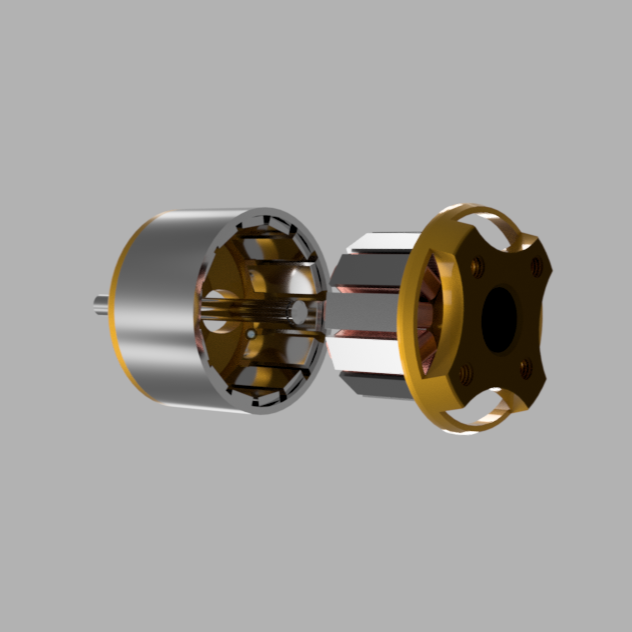
\includegraphics[width=5cm]{Renderizações/2 - BLDC.png}
        \caption{Motor BLDC Rotor}
        \footnotesize \textit{Fonte: Renderização própria no Fusion 360.}
        \label{2-BLDC}
    \end{figure}

    \begin{figure}[H]
        \centering
        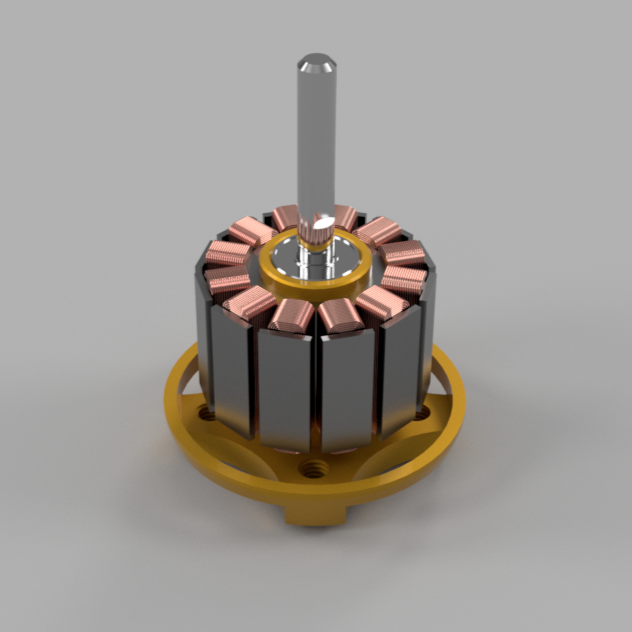
\includegraphics[width=5cm]{Renderizações/3 - BLDC.png}
        \caption{Motor BLDC Estator}
        \footnotesize \textit{Fonte: Renderização própria no Fusion 360.}
        \label{3-BLDC}
    \end{figure}

    \end{multicols}

\section{Conclusão}
    \noindent Ambos os motores se baseiam nos mesmos princípios físicos: a interação entre corrente elétrica e campo magnético gera forças que criam o torque necessário para o movimento 
    do rotor. No entanto, o BLDC se destaca pela precisão no controle da rotação, menor necessidade de manutenção e maior confiabilidade, sendo amplamente utilizado em aplicações modernas 
    que exigem alta performance e durabilidade.

\footnotetext[0]{Os Modelos de Inteligência Artificial só foram utilizados para verificação ortográfica e eventuais dúvidas relativas ao LaTeX}
\footnotetext[1]{As ditas "IA's" não foram utilizadas para validação dos fenômenos físicos descritos no documento}


%-------------------- Bibliografia --------------------%
\newpage
    
    \nocite{SEMESCOVA}
    \nocite{MOTRCC}
    \nocite{QUEROBOLSA}
    \nocite{BRASILESCOLA}
    \nocite{CORRENTEFOUCAULT}
    \nocite{LEIFARADAY}
    \nocite{MANUALLATEX}
    \nocite{pepadun}

    \bibliographystyle{apalike}
    \bibliography{ref}

%-------------------- Apêndicie --------------------%
\newpage 
\begin{appendices}

    \section{Uso de IA \textbf{Claude 4.0 Soneto}}
        \noindent Toda interação com o modelo está registrada no histórico de conversa. Devido ao documento estar muito longo optei por deixar essas interações no site oficial do modelo
        e disponibilizar o acesso através do link:
        \begin{quote}[H]
            \url{https://www.perplexity.ai/search/lt-apendicies-secoes-XNQBHhvyTcC.XS0I7rG3tQ}    
        \end{quote}
        
    \section{Modelos CAD Utilizados}
        \noindent Os modelos CAD utilizados neste trabalho foram obtidos gratuitamente na plataforma GrabCAD. Os arquivos foram empregados para ilustração e análise dos motores estudados. Os links para acesso direto aos modelos estão disponíveis abaixo:

        \begin{itemize}
            \item \textbf{Motor BLDC (A2212):}
            \begin{quote}
                \url{https://grabcad.com/library/a2212-bldc-motor-1}
            \end{quote}

            \item \textbf{Motor DC:}
            \begin{quote}
                \url{https://grabcad.com/library/dc-motor-191}
            \end{quote}
        \end{itemize}

        \noindent Todos os direitos e créditos relativos aos modelos pertencem aos respectivos autores na plataforma GrabCAD.


\end{appendices}
\end{document}
